\section{Additional results}
\label{app:sec:additional_exp}


\subsection{Ablation studies}
\label{app:sec:ablation_studies}

\textit{Module sensitivity:} We first compare the performance of \svdacro when it is applied to different modules (see trials 1-3).
Under consistent conditions, both individual MLP and attention updates improve performance, with MLP updates resulting in more pronounced gains.
Simultaneous updates to both module types yield even more significant enhancements.

\textit{Objective function:} We are interested in the performance impact from different objective functions, and we compare the RL objective with next-token prediction loss (see trials 2 and 4).
For the latter, we use instruction fine-tuning with official GSM8K solutions as target tokens.
Results show clear performance gains with RL, demonstrating its effectiveness in task-specific fine-tuning.
Conversely, next-token prediction even hinders performance.
This highlights RL's ability to handle cases lacking detailed solutions, suggesting its superiority in this context.

\textit{\svdacro vs LoRA:} Finally, we also evaluate LoRA using the RL objective (see trials 2 and 5).
A significant performance disparity is observed, primarily attributed to the severe instability of the LoRA training process.
Despite exploring a wide range of learning rates, LoRA's performance consistently lagged behind.
For further illustrations, see Figure~\ref{app:fig:lora_learning_curves} in the appendix.

\begin{table}[h]
% \begin{table}[!b]

% \vspace{-2mm}
\centering
\caption{\textbf{Ablation studies.} We fine-tune \llama on the GSM8K training split with different settings and the results on the test split along with zero-shot transfer results on MATH.
% We highlight the change in learning configurations for better visualization.
%Notably, we set the KL coefficient to 0.1 across all runs utilizing policy gradient for fair comparison.
}
% \vspace{-3.5mm}
% \small
% \begin{tabular}{llllccc}
% \toprule

% \textbf{\#} & \textbf{Method} & \textbf{Objective Function} & \textbf{Module} & \textbf{\#Params ($\downarrow$)} & \textbf{GSM8K ($\uparrow$)} & \textbf{MATH ($\uparrow$)} \\

% \midrule
% 0 & \multicolumn{4}{c}{\textsc{LLAMA-3-8B-Instruct}} & {75.89 {\scriptsize (\grey{1.00})}} & {24.54 {\scriptsize (\grey{1.00})}} \\ 
% \midrule

% 1 & \svdacro & Policy gradient & MLP & 0.39M & { 78.62 {\scriptsize (\green{1.04})}} & {24.20 {\scriptsize (\green{0.99})}} \\

% 2 & \svdacro & Policy gradient & \cellcolor{gray!20}{attention} & \textbf{0.16M} & {76.19 {\scriptsize (\green{1.00})}} & {24.20 {\scriptsize (\green{0.99})}} \\

% 3 & \svdacro & Policy gradient & \cellcolor{gray!20}{MLP + attention} & 0.58M & \textbf{{ 79.23 {\scriptsize (\green{1.04})}}} & \textbf{{25.04 {\scriptsize (\green{1.04)}}}} \\

% 4 & \svdacro & \cellcolor{gray!20}{Next token pred} & attention & \textbf{0.16M} & { 60.50 {\scriptsize (\green{0.80})}} & {18.52 {\scriptsize (\green{0.75})}} \\

% 5 & \cellcolor{gray!20}{LoRA} & Policy gradient & attention & 6.82M & { 57.92 {\scriptsize (\green{0.76})}} & {15.72 {\scriptsize (\green{0.64})}} \\

% \bottomrule
% \label{tab:res:ablation}
% \end{tabular}

% \vspace{-8mm}
% \end{table}

% \vspace{-3.5mm}
\small
\begin{tabular}{llllccc}
\toprule

\textbf{\#} & \textbf{Method} & \textbf{Objective Function} & \textbf{Module} & \textbf{\#Params ($\downarrow$)} & \textbf{GSM8K ($\uparrow$)} & \textbf{MATH ($\uparrow$)} \\

\midrule
0 & \multicolumn{4}{c}{\textsc{LLAMA-3-8B-Instruct}} & {75.89 {\scriptsize (\grey{1.00})}} & {24.54 {\scriptsize (\grey{1.00})}} \\ 
\midrule

1 & \svdacro & Policy gradient & MLP & 0.39M & { 78.62 {\scriptsize (\green{1.04})}} & {24.20 {\scriptsize (\green{0.99})}} \\

2 & \svdacro & Policy gradient & attention & \textbf{0.16M} & {76.19 {\scriptsize (\green{1.00})}} & {24.20 {\scriptsize (\green{0.99})}} \\

3 & \svdacro & Policy gradient & MLP + attention & 0.58M & \textbf{{ 79.23 {\scriptsize (\green{1.04})}}} & \textbf{{25.04 {\scriptsize (\green{1.04)}}}} \\

4 & \svdacro & Next token pred & attention & \textbf{0.16M} & { 60.50 {\scriptsize (\green{0.80})}} & {18.52 {\scriptsize (\green{0.75})}} \\

5 & LoRA & Policy gradient & attention & 6.82M & { 57.92 {\scriptsize (\green{0.76})}} & {15.72 {\scriptsize (\green{0.64})}} \\

\bottomrule
\label{tab:res:ablation}
\end{tabular}

\vspace{-5mm}
\end{table}



\subsection{Impact from number of few-shots}
\label{app:sec:ablation_few_shots}

We investigate the relationship between the number of samples available for few-shot adaptation and downstream performance.
Our analysis focused on the test task where \llama demonstrates the highest baseline performance, to prevent the potential for a null signal in our CEM-based search.


\begin{wraptable}{r}{0.5\textwidth}
\vspace{-4mm}
\caption{\textbf{Few-shot adaptation scaling.} Performance varies with number of examples.
}
% \vspace{-3.5mm}
\centering
\resizebox{0.45\textwidth}{!}{
\begin{tabular}{lc}
\toprule
\textbf{Method} & \textbf{ARC-Challenge} \\
\midrule
\llama & {\normalsize 80.63 {\footnotesize (\grey{1.00})}} \\
\midrule

\quad + 3-shot adaptation & {\normalsize 82.18 {\footnotesize (\green{1.02})}} \\
\quad + 5-shot adaptation & {\normalsize 82.38 {\footnotesize (\green{1.02})}} \\
\quad + 10-shot adaptation & \textbf{{\normalsize 82.61 {\footnotesize (\green{1.02})}}} \\
\quad + 20-shot adaptation & \textbf{{\normalsize 82.61 {\footnotesize (\green{1.02})}}} \\

\bottomrule
\end{tabular}}
\label{tab:ablation:few_shot_adaptation}
\vspace{-10mm}
\end{wraptable}


As Table~\ref{tab:ablation:few_shot_adaptation} shows, substantial benefits of our few-shot strategy are evident with as few as 3 to 5 test samples.
Moreover, performance appears to plateau beyond 10 samples, underscoring how our essential and inherently regularized \svdacro parameterization effectively complements self-adaptation.
This efficiency enables optimal use of data to enhance understanding of the test task.

\subsection{Cross-model svf transfer on the training tasks}
We provide complementary results to Table~\ref{tab:analysis:cross_model_main} in the main text, where we analyze the \svdacro cross-model transfer performance from training on GSM8K, MBPP-pro, and ARC-Easy to our considered test tasks. In Table~\ref{tab:analysis:cross_model_app}, we show the results in the same transfer setting this time evaluating \mistral on the same training tasks where the \llama \svdacro vectors were obtained from. Overall, we recognize a similar trend, albeit with less consistent improvement from the original model (only in 1 out of 3 tasks), but still much higher performance than the randomly shuffled baseline. These results further confirm that the canonical ordering of the \svdacro parameterization is key for cross-model transfer, highlighting once more its inherent suitability to empower self-adaptation.

\begin{table}[!h]
\caption{
\textbf{Cross-model $\boldsymbol{z}$ Vector Transfer.}
Results from transfering the SVF expert vectors trained on \llama to \mistral in the respective training tasks.}
\vspace{-3.5mm}
\centering
\begin{tabular}{lccc}
\toprule
\textbf{Method} & \textbf{GSM8K} & \textbf{MBPP-pro} & \textbf{ARC-Easy} \\
%\textit{SVF training task} & \small{\textit{GSM8K}} & \small{\textit{MBPP-pro}} & \small{\textit{ARC-Easy}} \\
\midrule

\textsc{Mistral-7B-Instruct-v0.3} & \textbf{{\normalsize 42.83 {\footnotesize (\grey{1.00})}}} & \textbf{{\normalsize 49.50 {\footnotesize (\grey{1.00})}}} & {\normalsize 81.65 {\footnotesize (\grey{1.00})}} \\

\midrule

\quad + Llama SVF (ordered $\sigma_i$) & {\normalsize 42.61 {\footnotesize (\red{0.99})}} & {\normalsize 48.48 {\footnotesize (\red{0.98})}} & \textbf{{\normalsize 81.78 {\footnotesize (\grey{1.00})}}} \\
\quad + Llama SVF (shuffled $\sigma_i$) & {\normalsize 41.93 {\footnotesize (\red{0.98})}} & {\normalsize 46.34 {\footnotesize (\red{0.94})}} & {\normalsize 80.81 {\footnotesize (\red{0.99})}} \\


\bottomrule
\end{tabular}
\label{tab:analysis:cross_model_app}
\end{table}

\subsection{Training curve of LoRA and policy gradient}

Figure~\ref{app:fig:lora_learning_curves} gives the learning curves for LoRA training on the GSM8K task.

\begin{figure}[h]
    \centering
    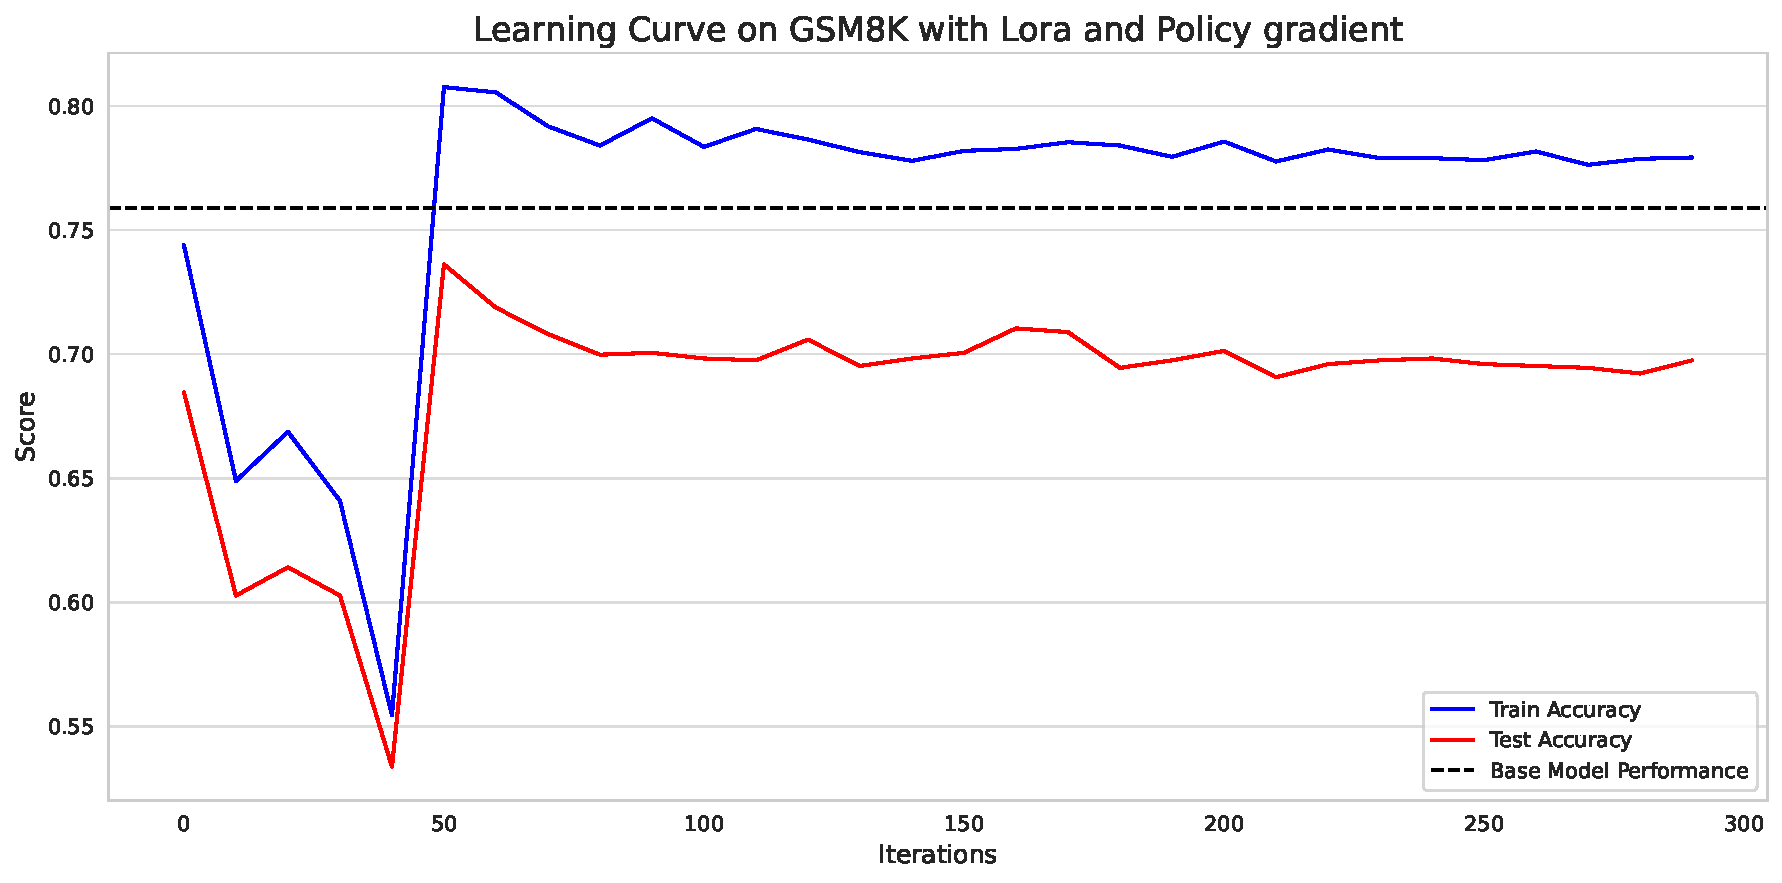
\includegraphics[width=0.6\textwidth]{images/lora_training_curve.pdf}
    \caption{\textbf{Training LoRA with policy gradient.} The dashed line shows the performance of \llama on the test split. LoRA collapses at the beginning of the training stage and fails to recover, leading to negative effects on test performance. We swept a wide range of learning rates $(2 \times 10^{-4}, 5 \times 10^{-4}, \dots, 2\times 10{-2}, 5\times 10^{-2})$, and all learning curves were similar to the one presented.}
    \label{app:fig:lora_learning_curves}
\end{figure}
